\chapter{Problemstellung}
\label{chap:formal}

% An dieser Stelle hat der cref Verweis leider nicht funktioniert, daher manueller Verweis

Zu Beginn des Studiums fällt es vielen Informatikstudierenden schwer, sich mit den Konzepten und Arbeitsweisen von Versionsverwaltungssystems vertraut zu machen (siehe Abschnitt 2.2).
Mögliche Ursachen hierbei sind beispielsweise fehlende Motivation und Zeit, sich außerhalb der Vorlesungen mit dem Thema auseinanderzusetzen.
Hinzu kommt oft ein Mangel an langfristigem Lerneffekt sowie technische Hürden, wie Probleme bei der Authentifizierung mit einem \gls{sshkey}.

\section{Mögliche Ursachen des Problemfeldes}
In der Vorarbeit zum Praxisprojekt wurden drei Hauptursachen für die genannten Schwierigkeiten identifiziert und analysiert.
Anschließend wurde eine Umfrage unter Studierenden der Fakultät 10 der Technischen Hochschule (TH) Köln durchgeführt, um diese Hypothesen zu überprüfen.

\subsection{Fehlende Motivation}
Eine Ursache könnte in der geringen Eigenmotivation der Studierenden liegen, sich mit dem Thema auseinanderzusetzen. So erscheint das Erlernen von Werkzeugen wie Git für einige möglicherweise als aktuell irrelevant für ihren Studienstand.
Viele Studierende verwenden zudem grafische Oberflächen in einer \gls{ide} wie Visual Studio Code, um \gls{git} und \gls{github} zu nutzen, ohne die zugrunde liegenden Funktionen wirklich zu verstehen. Dies könnte zu Bedienfehlern und Konflikten führen, beispielsweise wenn ein \gls{commit} Ablauf nicht korrekt durchgeführt wird.

\subsection{Fehlende langfristiger Lerneffekt}
Einige Studierende beschäftigen sich zwar selbstständig mit Git und GitHub, lesen jedoch lediglich Befehlsketten, ohne diese anzuwenden. 
Dadurch bleibt der langfristige Lerneffekt aus, und das grundlegende Verständnis der Konzepte von \gls{remote} und \gls{local} \gls{repository} wird oft vernachlässigt.

\subsection{Technische Probleme}
Eine weitere mögliche Ursache für den Wissensmangel sind technische Probleme. Manche Studierende haben keinen Zugriff auf einen Computer und können Git nur eingeschränkt nutzen.
Andere verfügen zwar über die notwendige Hardware, haben jedoch Schwierigkeiten bei der Einrichtung von Git, insbesondere der Authentifizierung via SSH-Key, was den Lernprozess erheblich behindert.

Die Umfrage ergab, dass fast alle genannten Faktoren von zehn oder mehr Studierenden als Hindernisse empfunden wurden. Technische Probleme wurden jedoch nur siebenmal als Grund genannt, und fehlende Hardware war für keinen der Teilnehmenden ein Problem.

\section{Prüfung der Thesen anhand einer Umfrage der Zielgruppe}
\label{sec:survey}
Zur Überprüfung der oben genannten Thesen wurde eine Umfrage unter den Studierenden der Fakultät 10 der TH Köln durchgeführt.
Der erste Teil der Umfrage sammelte demografische Daten der Teilnehmenden sowie Informationen zu ihren Erfahrungen mit den Versionsverwaltungssystemen Git und GitHub sowie gegebenenfalls weiteren Systemen.
Abschließend wurden die Studierenden nach ihrer Meinung zu einem möglichen Lernsystem befragt.

Die vollständigen Ergebnisse der Umfrage sind im Anhang dieses Berichts zu finden. Im Projektbericht selbst werden nur die Abschnitte der Umfrage ausgewertet, die für die jeweilige Problemstellung relevant sind.

Die Umfrage wurde in deutscher und englischer Sprache durchgeführt. Da die Fragen in beiden Versionen identisch waren, wurden die Ergebnisse zusammengeführt und gemeinsam ausgewertet.

\subsection{Git und GitHub Kenntnisse}
In der Umfrage sollten primär die Gründe für mögliche Wissensmängel ausgearbeitet werden.
Auf Grundlage dessen und der Wünsche der Studierenden sollte im weiteren Verlauf des Projektes dann ein System, zugeschnitten auf die Interessen der Zielgruppe, entwickelt werden.

Aus der Umfrage ließ sich schließen, dass alle Gründe, abgesehen von Hardwareproblemen, vergleichbar gleichmäßig ausgewählt wurden. Insgesamt konnte festgestellt werden, dass nicht nur Schwierigkeiten bestehen, sich die Kenntnisse selbst beizubringen, sondern auch ein Mangel an Studierenden, die Git über die Konsole direkt verwenden.
Relevant ist dies im Kontext, da über die grafischen Oberflächen möglicherweise die Zusammenhänge der Git-Kommandos nicht verstanden werden.

\begin{figure}[h!]
    \centering
    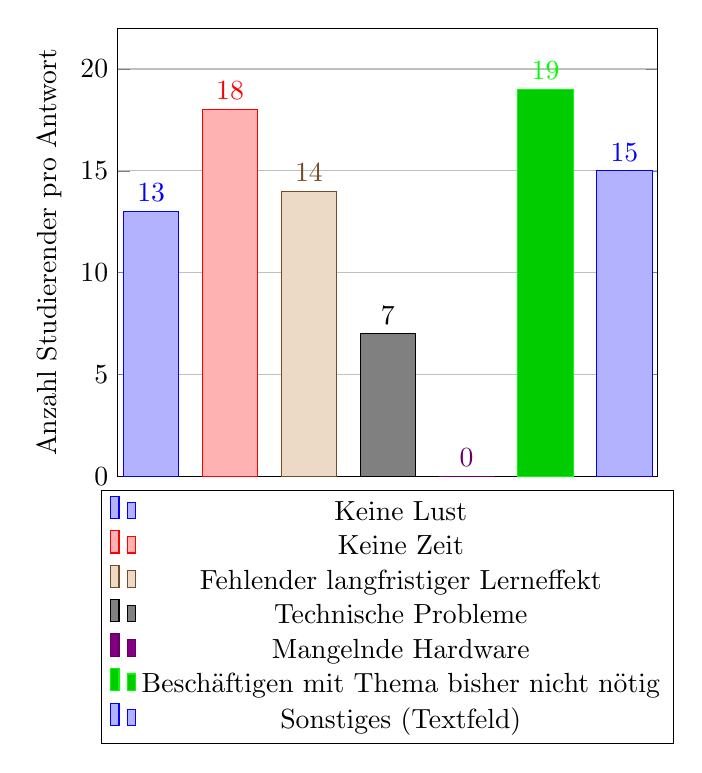
\begin{tikzpicture}
    \begin{axis}[
    	x tick label style={
    		/pgf/number format/1000 sep=},
    	ylabel=Anzahl Studierender pro Antwort,
    	enlarge x limits=2,
        ymax=22,
        ymin=0,
    	legend style={at={(0.5,-0.03)},
        anchor=north,legend columns=1},
        ybar,
        bar width=20pt,
        xticklabels={},
        xtick=\empty,
        nodes near coords,
        grid=major,
    ]
    \addplot coordinates {(1,13)};
    \addplot coordinates {(2,18)};
    \addplot coordinates {(3,14)};
    \addplot coordinates {(4,7)};
    \addplot coordinates {(5,0)};
    \addplot coordinates {(6,19)};
    \addplot coordinates {(7,15)};
    
    \legend{Keine Lust, Keine Zeit, Fehlender langfristiger Lerneffekt, Technische Probleme, Mangelnde Hardware, Beschäftigen mit Thema bisher nicht nötig, Sonstiges (Textfeld)}
    \end{axis}
\end{tikzpicture}
    \caption{Grafische Darstellung der Ergebnisse zur Frage: Mögliche Gründe für Wissensmängel im Bereich}
\end{figure}

Generell bewerteten viele Studierende, trotz dessen, dass viele dieser Git bereits im Studium verwendet hatten, ihre Kenntnisse eher mittelmäßig bis niedrig.

\begin{figure}[h!]
    \centering
    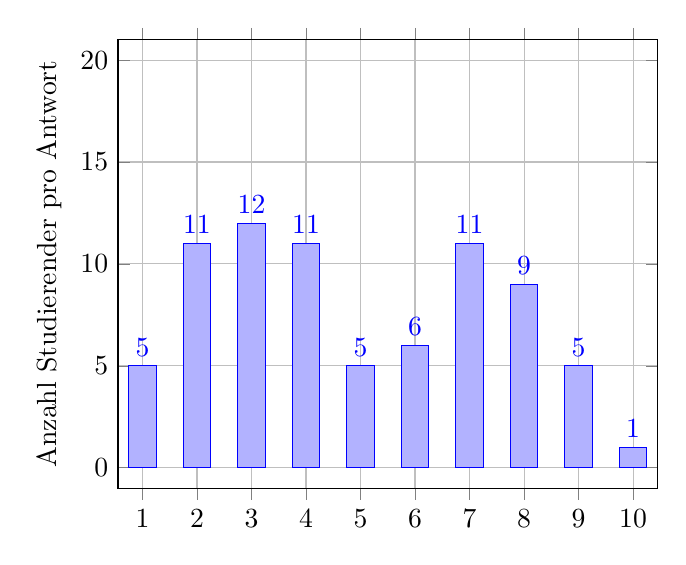
\begin{tikzpicture}
    \begin{axis}[
    	x tick label style={
    		/pgf/number format/1000 sep=},
    	ylabel=Anzahl Studierender pro Antwort,
    	enlargelimits=0.05,
        ymax=20,
        ymin=0,
    	ybar,
        xtick=data,
        xticklabels={1,2,3,4,5,6,7,8,9,10},
        grid=major,
        nodes near coords,
    ]
    \addplot 
    	coordinates {(1,5) (2,11)
    		  (3,12) (4,11) (5,5) (6,6) 
            (7,11) (8,9) (9,5) (10,1)};
    \end{axis}
\end{tikzpicture}
    \caption{Grafische Darstellung der Ergebnisse zur Frage: Wissen von Git}
\end{figure}

Die wichtigste Frage, die mit der Umfrage analysiert werden sollte, ist jedoch die zum Interesse des Systems. 
Durch die Ergebnisse hat sich herausgestellt, dass die Mehrheit der Befragten generell ein Interesse an einem Lernsystem zum Thema Git und GitHub hätte.

\begin{figure}[h!]
    \centering
    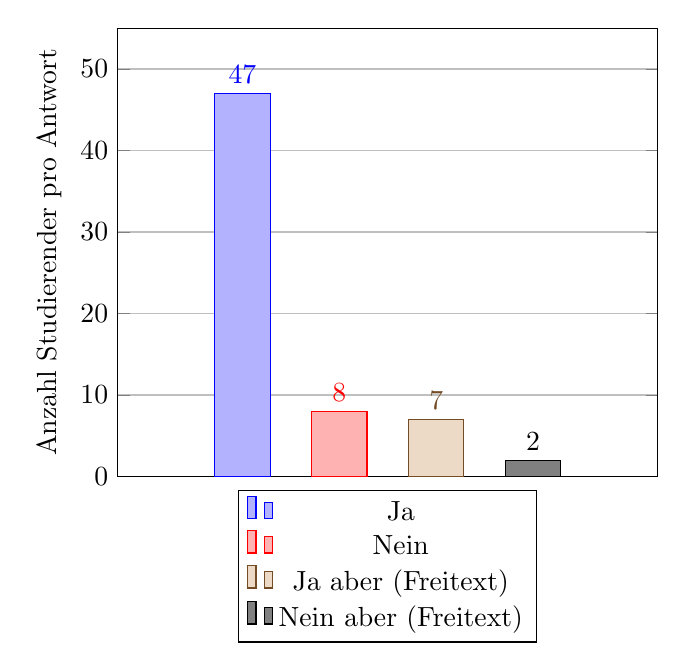
\begin{tikzpicture}
    \begin{axis}[
        x tick label style={
    		/pgf/number format/1000 sep=},
    	ylabel=Anzahl Studierender pro Antwort,
    	enlarge x limits=2,
        ymax=55,
        ymin=0,
    	legend style={at={(0.5,-0.03)},
        anchor=north,legend columns=1},
        ybar,
        bar width=20pt,
        xticklabels={},
        xtick=\empty,
        nodes near coords,
        grid=major,
    ]
    \addplot coordinates {(1,47)};
    \addplot coordinates {(2,8)};
    \addplot coordinates {(3,7)};
    \addplot coordinates {(4,2)};
    
    \legend{Ja, Nein, Ja aber (Freitext), Nein aber (Freitext)}
    \end{axis}
\end{tikzpicture}
    \caption{Grafische Darstellung der Ergebnisse zur Frage: Interessen an einem Lernsystem}
\end{figure}

Zudem ergab sich, dass tiefergehende Lerninhalte generell als wichtiger eingestuft wurden, als ein interessantes Setting mit ansprechendem Humor zu haben.
Im Kontext des Projektes hatte dies zunächst wenig Einwirkung, da der Prototyp um das Konzept der Koch-Analogie strukturiert wurde.

\begin{figure}[h!]
    \centering
    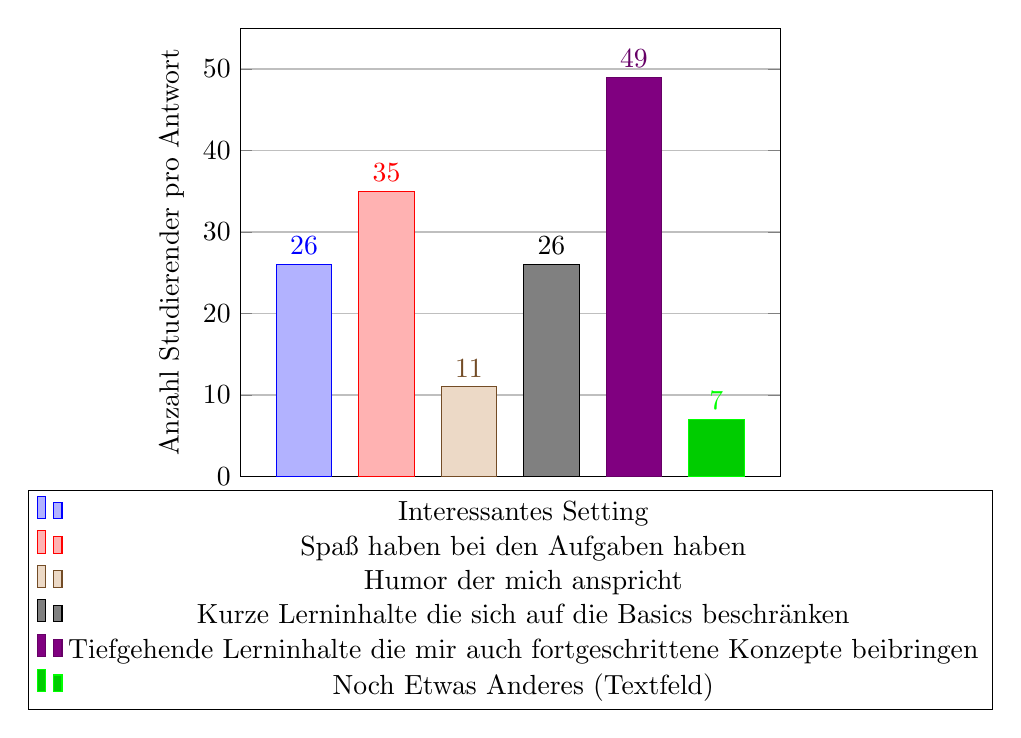
\begin{tikzpicture}
    \begin{axis}[
        x tick label style={
    		/pgf/number format/1000 sep=},
    	ylabel=Anzahl Studierender pro Antwort,
    	enlarge x limits=2,
        ymax=55,
        ymin=0,
    	legend style={at={(0.5,-0.03)},
        anchor=north,legend columns=1},
        ybar,
        bar width=20pt,
        xticklabels={},
        xtick=\empty,
        nodes near coords,
        grid=major,
    ]
    \addplot coordinates {(1,26)};
    \addplot coordinates {(2,35)};
    \addplot coordinates {(3,11)};
    \addplot coordinates {(4,26)};
    \addplot coordinates {(5,49)};
    \addplot coordinates {(6,7)};
    
    \legend{Interessantes Setting, Spaß haben bei den Aufgaben haben, Humor der mich anspricht, Kurze Lerninhalte die sich auf die Basics beschränken, Tiefgehende Lerninhalte die mir auch fortgeschrittene Konzepte beibringen, Noch Etwas Anderes (Textfeld)}
    \end{axis}
    \end{tikzpicture}
    \caption{Grafische Darstellung der Ergebnisse zur Frage: Wünsche an einem Lernsystem}
\end{figure}

Nähere Details zu den Antworten in den Freitextfeldern, sowie die restlichen Inhalte der Umfrageergebnisse befinden sich im Anhang des Projektberichtes.
